\documentclass[a4paper,12pt,twoside,openright]{book} 
%\usepackage[spanish, es-ucroman]{babel}
\usepackage[english]{babel}
\usepackage[utf8]{inputenc}
%\usepackage{fancyhdr}
%\usepackage{graphicx}
%\usepackage[inner=3.0cm,outer=2.5cm,top=3cm,bottom=3cm]{geometry}
%\usepackage{hlundef}
%\usepackage{tesis}
\usepackage[printonlyused]{acronym}
\usepackage{breakcites}
\usepackage{color,soul}
\usepackage{ae}
\usepackage[usenames,dvipsnames,table,xcdraw]{xcolor}
\usepackage{amsmath}
\usepackage{multirow}
\usepackage[inline]{enumitem}
\usepackage{tikz,pgfplots,pgfplotstable}
\usepackage{capt-of}
\usepackage{csvsimple}

\usepackage{caption}
\usepackage{subcaption}
\usepackage{booktabs}
\usepackage{enumitem}
\usepackage[colorinlistoftodos]{todonotes}
\usepackage{mathrsfs}
\newtheorem{proposicion}{Proposición}[section]
\usepackage{amsfonts}
\usepackage{amssymb}
\usepackage{xspace}
\usepackage{array}
\usepackage{etoolbox}
\usepackage[group-separator={,}]{siunitx}

\usepackage{import}


\usepackage{booktabs}
\newcommand{\ra}[1]{\renewcommand{\arraystretch}{#1}}

\setcounter{secnumdepth}{3}

\usepackage{filecontents,pgfplots,pgfplotstable}
\pgfplotsset{compat=1.13}
\usepgfplotslibrary{colormaps}

\usepackage{sidecap}
\sidecaptionvpos{figure}{b}
\sidecaptionvpos{table}{b}

\usepackage{natbib}
\setcitestyle{round}
%\bibliographystyle{apabrahand}
\usepackage[colorlinks=true]{hyperref}
\hypersetup{citecolor=blue}
\hypersetup{urlcolor=red}
\hypersetup{linkcolor=purple}

\usepackage{tikz-qtree}
\usepackage{arydshln}
\usetikzlibrary{shapes.geometric, arrows, decorations.pathreplacing, shadows,trees, positioning, calc, tikzmark, spy, mindmap, matrix}
\tikzstyle{roundedFrame} = [rectangle, text centered, rounded corners, draw=gray]
\tikzstyle{input} = [rectangle,text centered, draw=none]
\tikzstyle{emptyFrame} = [rectangle,text centered, draw=white]
\tikzstyle{frame} = [rectangle, text centered, draw=gray]
\tikzstyle{arrow} = [thick,->,>=stealth]

\usepackage{pifont} % DING


%%%%%%%%%%% Extra commands %%%%%%%%%%%%%%
\newcommand{\myparagraph}[1]{\smallskip\noindent\textbf{#1}\space}
\newcommand{\ie}{\textit{i.e.},\xspace}
\newcommand{\eg}{\textit{e.g.},\xspace}
\newcommand{\ea}{\textit{et al.}\xspace}
\newcommand{\etc}{\textit{etc.}}

\definecolor{pastelblue}{rgb}{0.68, 0.78, 0.81}
\definecolor{pastelorange}{rgb}{1.0, 0.7, 0.28}
\definecolor{pastelyellow}{rgb}{0.99, 0.99, 0.59}
\definecolor{pastelred}{rgb}{1.0, 0.41, 0.38}
\definecolor{pastelgreen}{rgb}{0.47, 0.87, 0.47}
\definecolor{error}{rgb}{1.0, 0.41, 0.38} % red
\definecolor{note}{rgb}{0.99, 0.99, 0.59} % yellow
\definecolor{info}{rgb}{0.68, 0.78, 0.81} % blue
\definecolor{tip}{rgb}{0.47, 0.87, 0.47} % green

\addto\extrasenglish{%
  \renewcommand{\chapterautorefname}{Chapter}%
  \renewcommand{\sectionautorefname}{Section}%
}

\hyphenation{fi-gu-re}
\hyphenation{le-gend}
\hyphenation{i-ma-ges}
\hyphenation{i-ma-ge}
\hyphenation{va-lues}
\hyphenation{va-lue}
\hyphenation{bet-ween}
\hyphenation{a-chie-ving}


\pagenumbering{Roman} 

\title{Safe and near optimal controller synthesis for \\Switched Systems}
\author{Richard Valentín Yantas Alcantara}
\orientador{PhD. Marco Muñiz}
\jurado
{
%\\ Dr. David Menotti -- Universidade Federal do Paraná  -- Brasil
%\\ Dr. Juan Carlos Gutierrez -- Universidad Católica San Pablo -- Perú
%\\ Dr. Erick Gomez Nieto -- Universidade de Sao Paulo -- Brasil
%\\ Dr. Alex Cuadros Vargas -- Universidad Católica San Pablo -- Perú
}

\dedicado{
%Aquí deberás colocar a quien va dedicada tu tesis por ejemplo: A Dios, por todo lo que me ha dado, a todos los profesores por sus enseñanzas y algunos amigos.
To my parents, Mario and Maria, who never stop giving of themselves in countless ways.
To my brothers and sister, who encourage and support me.
}

\begin{document}
\maketitle 

%mayores detalles de como usas las abreviaturas (acronimos)
% vea: http://www.ctan.org/tex-archive/macros/latex/contrib/acronym/
% hay un manual en pdf en esa misma direccion

\chapter*{Abbreviations}

\begin{acronym}
\acro{CNN}{Convolutional Neural Network}
\acro{CSV}{Comma-Separated Values}
\acro{GIS}{Geographic Information System}
\acro{HMM}{Hidden Markov Model}
\acro{JSON}{JavaScript Object Notation}
\acro{ML}{Machine Learning}
\acro{MSE}{Mean Squared Error}
\acro{MST}{Minimal Spanning Tree}
\acro{NLP}{Natural Language Processing}
\acro{OCR}{Optical Character Recognition}
\acro{RBF}{Radial Basis Function}
\acro{SVG}{Scalable Vector Graphics}
\acro{SVM}{Support Vector Machine}
\end{acronym}

\begin{agradecimientos}

First and foremost, I want to thank God for having guided me throughout these two years of study.

I would like to thank my family for their continuous support and encouragement during these years of study.

I would like to thank in a special way to the National Council for Science, Technology and Technological Innovation (CONCYTEC-PERU) and to the National Fund for Scientific Development, Technological and Technological Innovation (FONDECYT-CIENCIACTIVA), which through the Management Agreement 234-2015-FONDECYT have allowed the grant and financing of my studies in the Master Program in Computer Science at Universidad Cat\'{o}lica San Pablo (UCSP).

I would like to express my gratitude and appreciation to my advisor Jorge Poco for giving his guidance and support throughout the Master program and the preparation of this thesis.

%I also would like to take this opportunity to say warm thanks to all my beloved friends, who have been so supportive along the way of doing this thesis.

Finally, I thank all the people who directly or indirectly helped me in the preparation and presentation of this work, either by exchanging ideas, giving me advice and recommendations or by encouraging me to continue.


\end{agradecimientos}

\begin{abstract}
%----Image Teaser----%


%\begin{figure}[!h]
%    \begin{center}
%        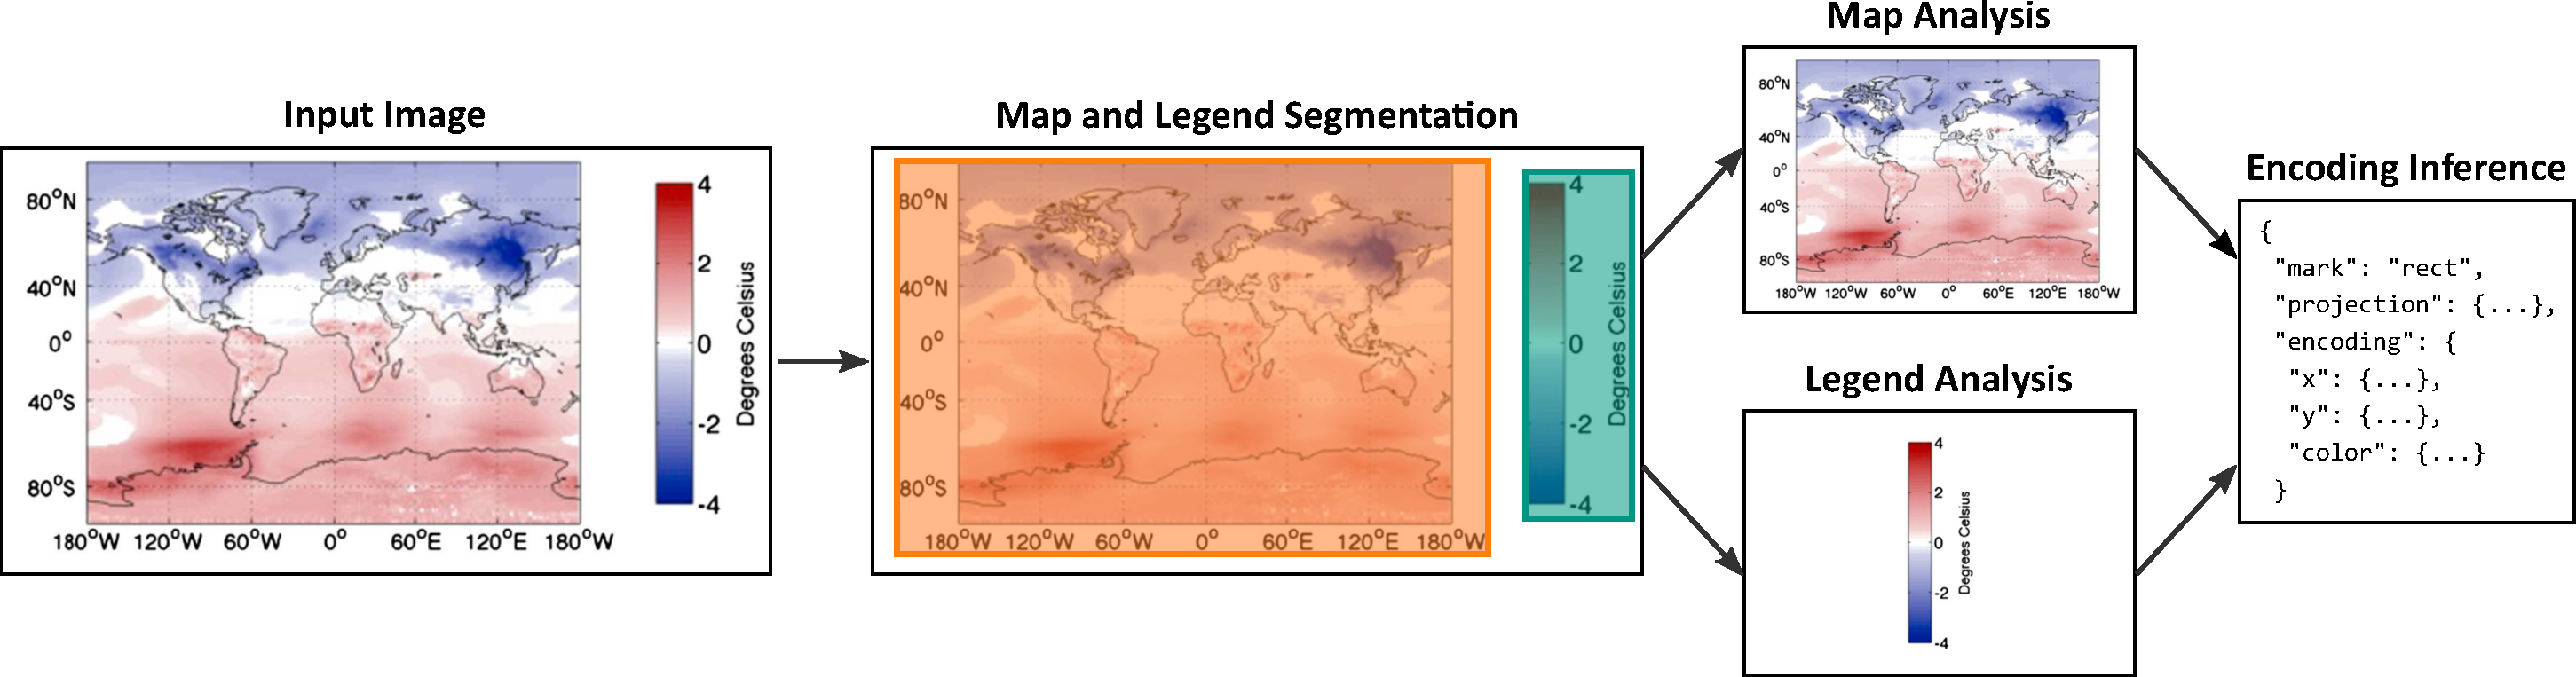
\includegraphics[width=\textwidth]{images/abstract_fig}
%    \end{center}
%\end{figure}

Switched systems are used in hybrid systems that are most common in engineering applications(\eg logic-dynamic controllers, internet congestion even physical systems with impact,\etc). Hybrid systems have been used to model several cyber-physical systems.

In This work, we propose a pipeline to solve switched systems, providing safety and optimal functions to different cyber-physical systems, we propose a solar water heating as a case of study.We evaluate our results comparing with traditional controllers. In addition, we present a system called UPPAL STRATEGO that will be used in this work.

\begin{flushleft}
\textbf{Keywords:} Control Theory, Game Theory,  Machine Learning, Model Checking.
\end{flushleft}

\end{abstract}

\begin{resumen}
Las visualizaciones de mapas son usadas en diferentes \'{a}reas para mostrar datos geogr\'{a}ficos (por ejemplo, datos climatológicos u oceanogr\'{a}ficos, resultados de análisis empresariales, entre otros). 
Estas visualizaciones se pueden encontrar en art\'{i}culos de noticias, art\'{i}culos cient\'{i}ficos y en la Web; sin embargo, muchas de ellas est\'{a}n disponibles como im\'{a}genes \textit{bitmap}, lo que dificulta que el computador interprete los datos visualizados para su indexaci\'{o}n y reutilizaci\'{o}n.

En este trabajo proponemos un \textit{pipeline} para recuperar la codificación visual a partir de im\'{a}genes \textit{bitmap} de mapas geogr\'{a}ficos que utilizan el color para codificar los valores de los datos. 
Nuestros resultados fueron analizados usando mapas extra\'{i}dos de documentos cient\'{i}ficos, logrando una alta precisi\'{o}n en cada paso del \textit{pipeline}. 
Adicionalmente presentamos a iGeoMap, nuestro sistema web que utiliza la codificaci\'{o}n visual extra\'{i}da para permitir la interacción del usuario sobre im\'{a}genes \textit{bitmap} de visualizaciones de mapas.

\begin{flushleft}
\textbf{Palabras clave:} Codificaci\'{o}n visual, Interpretaci\'{o}n de mapa, Visualizaci\'{o}n de mapa.
\end{flushleft}

\end{resumen}
 

\tableofcontents 
\listoftables 
\addcontentsline{toc}{chapter}{List of Tables}
%\cleardoublepage
\listoffigures 
\addcontentsline{toc}{chapter}{List of Figures}
%\listoftables 
%\listoffigures 

%%%%%%%%%%%%%%%%%%%%%%%%%%%%%%%%%%%%%%%%%%%%%%%%%%%%%%%%%%%%%%%%%%%%%
%%%%   En esta parte deberas incluir los archivos de tu tesis   %%%%%
%%%%%%%%%%%%%%%%%%%%%%%%%%%%%%%%%%%%%%%%%%%%%%%%%%%%%%%%%%%%%%%%%%%%%

\clearpage 
\pagenumbering{arabic} 


%-------------------------------------------------------------------------
% Background
%-------------------------------------------------------------------------
\newcommand{\figDefLatLon}{
\begin{figure}[!ht]
   \centering
   \begin{subfigure}{0.3\textwidth}
        \centering
     \includegraphics[scale=0.6]{images/def_latitude}
     \caption{Latitude.}
     \label{fig:def:lat}
   \end{subfigure} \ \ \
   \begin{subfigure}{0.3\textwidth}
        \centering
     \includegraphics[scale=0.6]{images/def_longitude}
     \caption{Longitude.}
     \label{fig:def:lon}
   \end{subfigure} \ \ \
   \begin{subfigure}{0.3\textwidth}
        \centering
     \includegraphics[scale=0.4]{images/def_graticule}
     \caption{Graticule.}
     \label{fig:def:graticule}
   \end{subfigure}
   \caption[Meridians, parallels, latitude, longitude and graticule.]{Meridians, parallels, latitude, longitude and graticule. (\subref{fig:def:lat}) Parallels are the imaginary lines parallel to the Equator and latitude is the distance between one parallel to the Equator. (\subref{fig:def:lon}) Meridians are imaginary lines that connect the poles and longitude is the distance between one meridian to the Greenwich meridian (both figures adapted from \url{https://iepbachillerato.wordpress.com/latitud-y-longitud/}).  (\subref{fig:def:graticule}) The graticule displays both parallels and meridians (from \url{http://desktop.arcgis.com/en/arcmap/10.3/map/page-layouts/what-are-grids-and-graticules-.htm}).}
   \label{fig:def:latlon}
\end{figure}
}

\newcommand{\figDefProj}{
\begin{figure}[!ht]
  \centering
  \includegraphics[width=0.6\textwidth]{images/def_projections}
  \caption[Transformation of the Earth's surface into a 2D plane.]{A map projection is the transformation of the Earth's surface into a 2D plane (adapted from \url{https://gistbok.ucgis.org/bok-topics/map-projections}).}
  \label{fig:def:projection}
\end{figure}
}

\newcommand{\figDefProjSamples}{
\begin{figure}[!ht]
   \centering
   \begin{subfigure}{0.48\textwidth}
     \includegraphics[height=4.5cm]{images/proj_equi}
     \caption{Equirectangular projection.}
     \label{fig:def:selprojs:equi}
   \end{subfigure} \ \ \
   \begin{subfigure}{0.48\textwidth}
     \centering
     \includegraphics[height=4.5cm]{images/proj_miller}
     \caption{Miller projection.}
     \label{fig:def:selprojs:miller}
   \end{subfigure} \ \ \
   \begin{subfigure}{0.48\textwidth}
     \includegraphics[height=4.5cm]{images/proj_robin}
     \caption{Robinson projection.}
     \label{fig:def:selprojs:robin}
   \end{subfigure}
   \caption[Map projections used in this work.]{Map projections used in this work. (\subref{fig:def:selprojs:equi}) Meridians and parallels in the Equirectangular projection are equally spaced straight parallel lines. (\subref{fig:def:selprojs:miller}) In Miller projection, the parallels are unequally spaced, closest near the Equator. (\subref{fig:def:selprojs:robin}) Robinson projection has elliptical arcs as meridians and the distance between parallels decreases near to the poles. These figures were generated by Basemap Toolkit~\citep{Whitaker2016}}
   \label{fig:def:selprojs}
\end{figure}
}

\newcommand{\figDefColormaps}{
\begin{figure}[!ht]
  \centering
  \includegraphics[width=\textwidth]{images/colormap_types}
  \caption[Examples of colormap types.]{Examples of colormap types that show three classes of colormaps: categorical, sequential and diverging. Depending on the data nature, colormaps can be quantized or continuous. (a) - (c) were generated by ColorBrewer (\url{http://colorbrewer2.org/}), and (d), (e) were retrieved from the user's guide of Matplotlib (\url{https://matplotlib.org/users/colormaps.html}).}
  \label{fig:def:colormaps}
\end{figure}
}


%-------------------------------------------------------------------------
% Dataset
%-------------------------------------------------------------------------
\newcommand{\figDataset}{
\begin{figure}[!ht]
  \centering
  \includegraphics[width=\columnwidth]{images/dataset}
  \caption[Examples of map visualization images from our corpus.]{Examples of map visualization images from our corpus, covering three projections and two color legend types. We extracted map images from geoscience journals in the field of climate change.}
  \label{fig:dataset}
\end{figure}
}


%-------------------------------------------------------------------------
% Annotations
%-------------------------------------------------------------------------
\newcommand{\figAnnotationsMap}{
\begin{figure}[!ht]
    \centering
    \includegraphics[width=0.5\textwidth]{images/annotation-map}
    \caption[Annotation in the map region.]{The internal elements of a map region include the map location (orange rectangle) and the textual elements representing latitude (red boxes), longitude (blue boxes), or other text.}
    \label{fig:ann:map}
\end{figure}
}

\newcommand{\figAnnotationsLegend}{
\begin{figure}[!ht]
   \centering
   \begin{subfigure}{0.48\textwidth}
     \includegraphics[width=\linewidth]{images/annotation-leg-cont}
     \caption{Annotation in continuous color legend.}
     \label{fig:ann:leg:cont}
   \end{subfigure}
   \begin{subfigure}{0.48\textwidth}
     \includegraphics[width=\linewidth]{images/annotation-leg-quant}
     \caption{Annotation in quantized color legend.}
     \label{fig:ann:leg:quant}
   \end{subfigure}
   \caption[Annotation in the legend region.]{For both legend types the color bar location (green rectangle) and the textual elements such as labels (red boxes) or other texts are annotated. (\subref{fig:ann:leg:cont}) The minimum and maximum pixel coordinates (yellow circles) are annotated in a continuous color legend; the red line represents all the colors inside the color bar. (\subref{fig:ann:leg:quant}) Representative pixels for each bin (yellow circles) are annotated in a quantized color legend.}
   \label{fig:ann:leg}
\end{figure}
}


%-------------------------------------------------------------------------
% Overview
%-------------------------------------------------------------------------
\newcommand{\figOverview}{
\begin{figure*}[!ht]
  \centering
  \includegraphics[width=\textwidth]{images/pipeline_overview}
  \caption[Four main steps of our approach to analyze an input map visualization.]{Our approach to analyzing an (a) input map visualization is comprised of four main steps: (b) We segment the image into map and legend regions. (c) The map region is analyzed to extract spatial encoding information. (d) The legend region is processed to extract color encoding information. (e) Finally, we combine the information extracted in the previous steps to infer a visual encoding specification.}
  \label{fig:overview}
\end{figure*}
}


%-------------------------------------------------------------------------
% Map and legend segmentation
%-------------------------------------------------------------------------
\newcommand{\figMapLegSegmentation}{
\begin{figure}[!ht]
   \centering
   \begin{subfigure}{0.46\textwidth}
     \includegraphics[width=\linewidth]{images/region_seg_02}
     \caption{Grayscale image of \autoref{fig:overview}a.}
     \label{fig:maplegseg:gray}
   \end{subfigure} \ \ 
   \begin{subfigure}{0.46\textwidth}
     \includegraphics[width=\linewidth]{images/region_seg_03}
     \caption{Binary image.}
     \label{fig:maplegseg:binary}
   \end{subfigure} \\
   \begin{subfigure}{0.46\textwidth}
     \includegraphics[width=\linewidth]{images/region_seg_04}
     \caption{Flood fill the holes.}
     \label{fig:maplegseg:fill}
   \end{subfigure} \ \ 
   \begin{subfigure}{0.46\textwidth}
     \includegraphics[width=\linewidth]{images/region_seg_05}
     \caption{Image eroded.}
     \label{fig:maplegseg:erosion}
   \end{subfigure} \\
   \begin{subfigure}{0.46\textwidth}
     \includegraphics[width=\linewidth]{images/region_seg_06}
     \caption{The two largest connected components.}
     \label{fig:maplegseg:largest}
   \end{subfigure} \ \ 
   \begin{subfigure}{0.46\textwidth}
     \includegraphics[width=\linewidth]{images/region_seg_07}
     \caption{Components to determine the regions.}
     \label{fig:maplegseg:components}
   \end{subfigure}
   \caption[Steps to segment a map visualization into map and legend regions.]{Steps to segment a map visualization into map and legend regions.}
   \label{fig:maplegseg}
\end{figure}
}


%-------------------------------------------------------------------------
% Map Analysis
%-------------------------------------------------------------------------
\newcommand{\figMapAnalysis}{
\begin{figure*}[!ht]
  \centering
  \includegraphics[width=\columnwidth]{images/pipeline_mapAnalyzer}
  \caption[Pipeline of map analyzer to extract spatial information.]{Map analysis pipeline for extracting spatial information. (a) The map region is given as input. (b) We identify the text bounding boxes and (c) they are classified depending on their text role. Next, (d) we extract the text content and (e) infer the label values. Finally, (f) we infer the map projection type.}
  \label{fig:pipeline_mapAnalyzer}
\end{figure*}
}

\newcommand{\figMapTextBoxIdentify}{
\begin{figure}[!ht]
   \centering
   \begin{subfigure}{0.45\textwidth}
     \includegraphics[width=\linewidth]{images/mapAnalysis_textExtract_01}
     \caption{Binary image after removing map.}
     \label{fig:map:textboxiden:binary}
   \end{subfigure} \ \ 
   \begin{subfigure}{0.45\textwidth}
     \includegraphics[width=\linewidth]{images/mapAnalysis_textExtract_02}
     \caption{Connected components.}
     \label{fig:map:textboxiden:components}
   \end{subfigure} \\
   \begin{subfigure}{0.45\textwidth}
     \includegraphics[width=\linewidth]{images/mapAnalysis_textExtract_03}
     \caption{Bounding boxes of components.}
     \label{fig:map:textboxiden:bboxcom}
   \end{subfigure} \ \  
   \begin{subfigure}{0.45\textwidth}
     \includegraphics[width=\linewidth]{images/mapAnalysis_textExtract_04}
     \caption{\ac{MST} from bounding box centers.}
     \label{fig:map:textboxiden:mst}
   \end{subfigure} \\
   \begin{subfigure}{0.45\textwidth}
     \includegraphics[width=\linewidth]{images/mapAnalysis_textExtract_05}
     \caption{Isolated words after discarding edges.}
     \label{fig:map:textboxiden:deledges}
   \end{subfigure} \ \ 
   \begin{subfigure}{0.45\textwidth}
     \includegraphics[width=\linewidth]{images/mapAnalysis_textExtract_06}
     \caption{Merged words.}
     \label{fig:map:textboxiden:bboxes}
   \end{subfigure}
   \caption[Steps to identify text bounding boxes from a map region.]{Steps to identify text bounding boxes from the map region shown in \autoref{fig:pipeline_mapAnalyzer}a.}
   \label{fig:map:textboxiden}
\end{figure}
}

\newcommand{\figInferValue}{
\begin{figure}[!ht]
  \centering
  \includegraphics[width=0.8\textwidth]{images/mapAnalysis_inferValue}
  \caption[Analysis to determine the sign for the latitude/longitude value.]{Centers of text bounding boxes are sorted by $y$-coordinate if they are latitude type and by $x$-coordinate if they are longitude type. When latitude numbers decrease, they are positive, in other case are negative. In a similar way, when longitude numbers increase to 180 are positive but if are greater than 180 or decrease are negative.}
  \label{fig:map:inferval}
\end{figure}
}

\newcommand{\figInferProjection}{
\begin{figure}[!ht]
  \centering
  \includegraphics[width=\columnwidth]{images/mapAnalysis_inferProj}
  \caption[Map templates for each geo projection and their corresponding fit curves.]{Map templates for each geo projection and their corresponding fit curves. The curve fits points of the relationship between latitude values and their position into the map region; red points represent the distribution of latitudes and the blue curve represents the fit.}
  \label{fig:mapAnalyzer_inferProj}
\end{figure}
}

\newcommand{\figInferProjectionEx}{
\begin{figure}[!ht]
  \centering
  \includegraphics[width=\textwidth]{images/mapAnalysis_inferProj_ex}
  \caption[Example how the geo projection is inferred by our method.]{Example how the geo projection is inferred by our method. (a) Given an input map region, we compute the distribution of its latitudes. For each projection type, we compute $pos'_i$ using the corresponding fit curve and scale ratios $r_i$. (b), (c) and (d) show these computation for Equirectangular, Miller and Robinson projections, respectively.}
  \label{fig:map:inferproj_ex}
\end{figure}
}


%-------------------------------------------------------------------------
% Legend Analysis
%-------------------------------------------------------------------------
\newcommand{\figLegAnalysis}{
\begin{figure}[!ht]
  \centering
  \includegraphics[width=\columnwidth]{images/pipeline_legAnalyzer}
  \caption[Legend analysis pipeline for extracting color information.]{Legend analysis pipeline for extracting color information. (a) The legend region is given as input and (b) it is classified by type. Then (c) we identify the text bounding boxes, (d) classify them, (e) extract their text using \ac{OCR}, and finally (f) extract colors from the color bar.}
  \label{fig:pipeline_legAnalyzer}
\end{figure}
}

\newcommand{\figLegTextBoxIdentify}{
\begin{figure}[!ht]
   \centering
   \begin{subfigure}{0.155\textwidth}
     \centering
     \fbox{\includegraphics[width=0.7\linewidth]{images/legAnalysis_textExtract_01}}
     \caption{Binary image.}
     \label{fig:leg:textboxiden:binary}
   \end{subfigure} \ \ \
   \begin{subfigure}{0.155\textwidth}
     \centering
     \fbox{\includegraphics[width=0.7\linewidth]{images/legAnalysis_textExtract_02}}
     \caption{Connected components.}
     \label{fig:leg:textboxiden:components}
   \end{subfigure} \ \ \
   \begin{subfigure}{0.155\textwidth}
     \centering
     \fbox{\includegraphics[width=0.7\linewidth]{images/legAnalysis_textExtract_04}}
     \caption{\ac{MST} from centers.}
     \label{fig:leg:textboxiden:mst}
   \end{subfigure} \ \ \
   \begin{subfigure}{0.155\textwidth}
     \centering
     \fbox{\includegraphics[width=0.7\linewidth]{images/legAnalysis_textExtract_05}}
     \caption{Isolated words.}
     \label{fig:leg:textboxiden:deledges}
   \end{subfigure} \ \ \
   \begin{subfigure}{0.155\textwidth}
     \centering
     \fbox{\includegraphics[width=0.7\linewidth]{images/legAnalysis_textExtract_06}}
     \caption{Merged words.}
     \label{fig:leg:textboxiden:bboxes}
   \end{subfigure}
   \caption[Steps to identify text bounding boxes in the legend region.]{Steps to identify text bounding boxes in the legend region shown in \autoref{fig:pipeline_legAnalyzer}a.}
   \label{fig:leg:textboxiden}
\end{figure}
}

\newcommand{\figLegColorExtractQuan}{
\begin{figure}[!ht]
  \centering
  \includegraphics[width=0.47\textwidth]{images/legAnalysis_colorExtract_quan}
  \caption[Color extraction of quantized legends.]{Given a horizontal quantized legend, we compute the absolute values of its horizontal derivative; then $k$ peaks are identified to extract $k+1$ colors (yellow circles).}
  \label{fig:leg:colorextract:quan}
\end{figure}
}


%-------------------------------------------------------------------------
% Encoding Inference
%-------------------------------------------------------------------------
\newcommand{\figEncGeneration}{
\begin{figure}[!ht]
  \centering
  \includegraphics[width=.83\textwidth]{images/visenc_generation}
  \caption[Recovery of visual encoding using data extracted by map analyzer and legend analyzer.]{Recovery of visual encoding using data extracted by map analyzer and legend analyzer in a declarative grammar similar to Vega-Lite~\citep{Satyanarayan2017}. Some values are assigned directly (colored) and others need to be inferred using extracted data.}
  \label{fig:visenc_gen}
\end{figure}
}

\newcommand{\figVisEncColor}{
\begin{figure}[!ht]
   \centering
   \begin{subfigure}{0.31\textwidth}
     \includegraphics[width=\linewidth]{images/visenc_color_cont}
     \caption{Continuous.}
     \label{fig:visenc:color:cont}
   \end{subfigure} \ \
   \begin{subfigure}{0.31\textwidth}
      \includegraphics[width=\linewidth]{images/visenc_color_quanval}
     \caption{Quantized: color$\rightarrow$value.}
     \label{fig:visenc:color:quanval}
   \end{subfigure} \ \
   \begin{subfigure}{0.31\textwidth}
     \includegraphics[width=\linewidth]{images/visenc_color_quanran}
     \caption{Quantized: color$\rightarrow$range.}
     \label{fig:visenc:color:quanran}
   \end{subfigure}
   \caption[Variation of the color channel depending on the legend type.]{Variation of the color channel depending on the legend type. \texttt{range} entry is an array of hexadecimal colors and \texttt{domain} can be an array of values or tuples.}
   \label{fig:visenc:color}
\end{figure}
}


%-------------------------------------------------------------------------
% Application: Recoloring
%-------------------------------------------------------------------------
\newcommand{\figAppRecoloring}{
\begin{figure*}[!ht]
  \centering
  \includegraphics[width=0.65\textwidth]{images/app-recolor.pdf}
%  \vspace{-20pt}
  \caption[Automatic recoloring.]{Automatic recoloring: given a map visualization and a target color palette, we generate a new image that contains the recolored map visualization.}
  \label{fig:app:recolor}
%  \vspace{-10pt}
\end{figure*}
}

%-------------------------------------------------------------------------
% Application: Interactive Overlays
%-------------------------------------------------------------------------
\newcommand{\figAppOverlays}{
\begin{figure*}[!ht]
  \centering
  \includegraphics[width=\textwidth]{images/app-overlays.pdf}
 % \vspace{-20pt}
  \caption[Interactions using graphical overlays.]{Interactions using graphical overlays. Each row corresponds to a legend type. The second column shows highlights of the legend in response to selected areas in the map region. The third column illustrates highlights of the data in response to selected legend values.}
  \label{fig:app:overlays}
\end{figure*}
}

%-------------------------------------------------------------------------
% Application: Captions
%-------------------------------------------------------------------------
\newcommand{\figAppCaption}{
\begin{figure*}[!ht]
  \centering
  \includegraphics[width=\textwidth]{images/app-captions}
  \caption[Examples of captions generated using the output of our pipeline.]{Examples of captions generated using the output of our pipeline. These captions are generated using the text templates shown in \autoref{tab:textTemplates}. When there is nothing selected, the application shows a generic caption; however, when the user selects one or more regions, the caption is updated.}
  \label{fig:app:captions}
\end{figure*}
}

%-------------------------------------------------------------------------
% Application: Reprojections
%-------------------------------------------------------------------------
\newcommand{\figAppReprojection}{
\begin{figure}[!ht]
  \centering
  \includegraphics[width=0.65\textwidth]{images/app-reprojection}
  \caption[Examples of map reprojection.]{Examples of map reprojection: given a  bitmap image and a target map projection, we generate a new image that contains the reprojected map which maintains original data.}
  \label{fig:app:reprojection}
\end{figure}
}

%-------------------------------------------------------------------------
% Application: Data Extraction
%-------------------------------------------------------------------------
\newcommand{\figAppDataExt}{
\begin{figure}[!ht]
  \centering
  \includegraphics[width=0.65\textwidth]{images/app-dataExtraction}
  \caption[Analysis of extracted encoded data on map visualizations.]{Analysis of extracted encoded data on map visualizations. User can know how distribution of legend values is inside map area and which legend value is the most common.}
  \label{fig:app:dataextract}
\end{figure}
}


%-------------------------------------------------------------------------
% iGeoMap: modes
%-------------------------------------------------------------------------
\newcommand{\figIGMmodes}{
\begin{figure}[!ht]
   \centering
   \begin{subfigure}{0.48\textwidth}
     \includegraphics[width=\linewidth]{images/igeomap-mode-edit}
     \caption{Edition mode.}
     \label{fig:igeomap:modes:edit}
   \end{subfigure} \hspace{0.2cm}
   \begin{subfigure}{0.48\textwidth}
      \includegraphics[width=\linewidth]{images/igeomap-mode-interact}
     \caption{Interaction mode.}
     \label{fig:igeomap:modes:interact}
   \end{subfigure}
   \caption[Visualization modes in iGeoMap.]{Visualization modes in iGeoMap. (\subref{fig:igeomap:modes:edit}) The extracted data is visualized and can be modified when \textit{edition mode} is active. (\subref{fig:igeomap:modes:interact}) The available interactions appears at left side when the \textit{interaction mode} is active.}
   \label{fig:igeomap:modes}
\end{figure}
}

%-------------------------------------------------------------------------
% iGeoMap: GUI
%-------------------------------------------------------------------------
\newcommand{\figIGMview}{
\begin{figure}[!ht]
  \centering
  \includegraphics[width=0.75\textwidth]{images/igeomap-view}
  \caption{iGeoMap: a web-based system that uses the information extracted by our pipeline.}
  \label{fig:igeomap:view}
\end{figure}
}

\newcommand{\figIGMgui}{
\begin{figure}[!ht]
  \centering
  \includegraphics[width=0.9\textwidth]{images/igeomap-gui}
  \caption[Principal parts in user's interface of iGeoMap.]{Principal parts in user's interface of iGeoMap. In the tool panel, the user can change the visualization mode and choose an interaction type. At the middle, we have the interaction area and a viewer that displays additional information. Finally, the gallery shows sample images.}
  \label{fig:igeomap:gui}
\end{figure}
}

%-------------------------------------------------------------------------
% iGeoMap: implementation
%-------------------------------------------------------------------------
\newcommand{\figIGMdev}{
\begin{figure}[h!]
 \centering
 \includegraphics[scale=0.7]{images/igeomap-gui}
 \caption[Correspondencia entre colores y valores.]{Correspondencia entre colores y valores. (a) Imagen de entrada donde se encuentra el pixel $i$. (b) Escala de colores que tiene $N$ colores que serán evaluados con el color de $i$. (c) Vector $V$ usado en nuestro método secuencial. (d) Textura de posiciones generada como salida del \textit{fragment shader} en nuestro método paralelizado.}
 \label{fig:igeomap:dev}
\end{figure}
}
	% contain all images
\chapter{Introduction}
\label{ch:intro}

% In \autoref{sec:motivation} we describe the motivation and context of our work, \autoref{sec:problem} presents our problem statement. \autoref{sec:objectives} shows the objectives of this work. Finally, \autoref{sec:outline} describes the structure of this thesis document.


\section{Motivation and Context}
\label{sec:motivation}
%%%TODO: FALTA MAS TEXTO EN LA MOTIVATION

Switched systems are widely used in engineering applications and its importance has grown up considerably these last years, because of their ease of implementation for controlling cyber-physical systems.A switched systems is a set of dynamical systems, each with its own dynamical behaviour controlled by a parameter mode $u$ whose values are in a finite set $U$(See ~\cite{liberzon2003switching}). However, due to the composition of many switched systems together, the global switched systems has a number of modes and dynamics which increases exponentially. 

Switched systems have numerous applications in control of mechanical systems, the automotive industry, and many other fields. 

\section{Problem Statement}
\label{sec:problem}
Nowadays, there is a large number of methods to solve switched systems; however, it does not have guarantee in safety. For that reason, we propose a new approach to solve switched systems. 
\section{Objectives}
\label{sec:objectives}

\subsection*{General Objective}
Our main objective is to propose a pipeline to solve switched systems guarantee safety and optimal synthesis controllers. 

\subsection*{Specific Objectives}
To achieve our main objective, we have the following specific objectives:
\begin{itemize}
 \item Define a case of study and get its mathematical model.
 \item Implement a safety controller for switched systems.
 \item Optimize the switched systems using model checking techniques.
 \item Evaluate each step of the pipeline and compare with traditional approaches.
\end{itemize}


\section{Contributions}
This thesis proposes a novel approach to solve switched systems guaranteeing safety and optimal controller synthesis. This procedure to consider stochastic variables as an input for the system. Our contributions are related to each part and are detailed below.

\begin{itemize}
 \item Define a synthesis controller with the next:.
 
 \begin{itemize}
  \item We propose a method to guarantee safe controller. This methods consider three regions to have reachability and safety in the system.
  \item We also demonstrate the utility of the proposed method comparing with traditional methods.
 \end{itemize}
 \item Analyze the stability for our case of study study.
 \begin{itemize}
  \item analyze the zeros and poles for the system.
 \end{itemize}
\end{itemize}


\section{Outline}
\label{sec:outline}
This thesis document is divided into six chapters. After this introduction and problem formulation, in \autoref{ch:relatedWorks} we survey the literature about the recent research in safety controllers and optimal controller synthesis. \autoref{ch:background} presents some basic concepts about the dynamical systems, traditional controllers, switched systems,stability criteria and optimal controller technique. Next, in Chapter x we describe in detail the corpus, techniques used by our pipeline and their evaluation results. Finally, the limitations, future works, and conclusions of this work are presented in Chapter z.

\chapter{Related Works}
\label{ch:relatedWorks}
Our work draws on prior research in the areas of map interpretation that is focused on extracting information from maps, automatic chart interpretation focused on analyzing charts and interactive applications from chart images that enable user-interaction.


\section{Map Interpretation}
\label{sec:mapInterpretation}
Researchers have proposed various methods to perform automatic \textit{map interpretation} \citep{Walter2011} to extract information from maps and analyze their content. For instance, \citeauthor{Dhar2006}~\citep{Dhar2006} analyze scanned topographic maps to extract and recognize symbols (\eg trees, forests, rivers, cities, huts, \etc) and text contained within the map. One of the steps is to separate the image into four layers: green elements (trees, forests), red elements (streets), blue elements (rivers, lakes) and black elements (text). The map scale and range of latitude/longitude coordinates are entered by the user to locate points on the map given their geographical coordinates. Finally, the output is an \textit{e-map} that can be used as input to \ac{GIS}. \citeauthor{Pezeshk2011}~\citep{Pezeshk2011} also worked on scanned topographic maps; their purpose was to automatically extract each component of the map in separate layers and recognize the text contained. They propose an algorithm for extracting linear features to generate a layer containing map lines (streets, roads, \etc); they then use the RANSAC algorithm~\citep{Fischler1981} to improve the text preprocessing and a \ac{HMM} to recognize texts and generate a text output layer.

These previous works focus mainly on topographic maps --- \ie maps characterized by contour lines and road lines~\citep{Pezeshk2011} --- and recognizing their symbols. Our approach automatically extracts spatial information from the geographical map contained in a map visualization; this information includes the type of geographic projection used by the map and the range of latitude and longitude values in the displayed region.


\section{Automatic Chart Interpretation}
\label{sec:chartInterpretation}
A growing number of techniques focus on the ``inverse problem" of data visualization: given a visualization, recover the underlying visual encoding and its corresponding data values~\citep{Poco2017a}. Some of these approaches have focused on \emph{data extraction}. For instance, ReVision~\citep{Savva2011} classifies images by chart type and extracts data from pie and bar charts to output a relational data table. Similarly, the VIEW system~\citep{Gao2012} extracts information from raster-format charts (\eg pie, bar, and line charts). It first distinguishes graphical and textual connected-components; depending on the graphic type it applies a different approach to extract data; finally, it generates a data table with that information. \citeauthor{Al-Zaidy2016}~\citet{Al-Zaidy2016} propose a system that extracts data values from bitmap images of bar charts and generates a semantic graph using the label roles (\eg x-title, x-labels, y-title, \etc); then, the semantic graph is used to generate a summary that describes the input image.

FigureSeer~\citep{Siegel2016} is a framework that extracts information from line charts. It detects the axes to extract their labels and infers their scales through curve fitting. To perform legend analysis, it uses a random-forest classifier~\citep{randForest2001} to determine whether or not text serves as a legend label and then obtains its symbol. The analysis of the plotting area is done using \ac{SVM}~\citep{Cortes1995} and a \ac{CNN}~\citep{LeCun1998} to learn functions and avoid problems caused by the occlusion between the lines. Another application is ChartSense~\citep{Jung2017}, an interactive system for data extraction from five types of charts: line, area, radar, bar, and pie charts. Its first step is to classify chart images using a classifier based on GoogLeNet~\citep{googlenet2014}; it then extracts the data using optimized extraction algorithms for each chart type. 
% 
These approaches extract data from charts that contain discrete legends (\eg bar, pie, area, line, or radar charts). Our work is focused on the extraction of data from visual components in map visualizations that contain continuous and quantized color legends. This chart type has not been addressed so far, despite being considered in ReVision~\citep{Savva2011} during its classification step.

On the other hand, some methods have been focused on \textit{recovering visual encoding} from a chart. \citeauthor{Harper2014}~\citep{Harper2014} present a tool to decompose and redesign visualizations created with the D3 library~\citep{Bostock2011} (\eg bar charts, line charts, scatter plots, donut charts, and choropleth). This tool extracts data, marks, and visual encoding by analyzing the \ac{SVG} elements of the chart and the data bound to those elements via JavaScript.
\citeauthor{Poco2017}~\citep{Poco2017} propose a method to recover visual encodings from bitmap images of bar charts, area charts, line charts, and scatter plots; their pipeline identifies textual elements in the image, determines their role within the chart (\eg chart title, $x$-labels, $x$-title, \etc), and recovers the text content using \ac{OCR}. They also trained a \ac{CNN}~\citep{LeCun1998} for classifying 10 chart types, which achieved an average accuracy better than ReVision and ChartSense, achieving an accuracy of 96\% for classifying maps. Using this extracted information they then recover a visual encoding specification. However, their work does not include extraction of color encodings or geographic projections.

As part of this thesis, we presented a work~\citep{Poco2017a} where we proposed a technique to extract the color encoding from discrete and continuous legends of chart images, including geographic maps. We identify the colors used and the legend texts, then recover the full color mapping (\ie associating value labels with their corresponding colors). We continue our thesis work upon that approach focusing on map visualizations; thus, we had to tackle other challenges (such as identifying map projections) and develop new applications enabled by our map image analysis pipeline.


\section{Interactive Applications from Chart Images}
\label{sec:intApps}
% FROM qualification doc (translate)
The extracted information from chart images can be useful for different applications. For instance, ReVision~\citep{Savva2011} has an interface to redesign the input chart based on the relational data table extracted by its pipeline. \citeauthor{Kong2012}~\citep{Kong2012} propose to create interactive overlays that are placed above chart bitmap images using the extracted data by ReVision~\citep{Savva2011} and Datathief \citep{Tummers2006} pipelines to improve the chart reading.

\citeauthor{Kong2014}~\citep{Kong2014} developed an interactive document viewer to improve the reading experience, in this application the user can select a paragraph in a document and some components in the charts are highlighted depending on the selection; they use ReVision~\citep{Savva2011} to extract data from bar charts and a manual annotation interface to recover the original data for other chart types. Other works like ChartSense~\citep{Jung2017} and iVoLVER~\citep{Mendez2016} use semi-automatic approaches to extract data values and also present interactive annotation interfaces to correct the output data and improve the interpretation of charts.

In the same way, we propose a web-based system named iGeoMap that enables the user-interaction on bitmap images of map visualizations. iGeoMap uses the visual encoding generated by our pipeline to create interactive overlays, generate automatic captions, recolor and reproject the input map visualization.


\section{Final Considerations}
This chapter presented some recent proposals related to our thesis work. Some research works have been focused on analyzing topographic maps to extract symbols and texts. On the other hand, other works have focused on extracting data from chart images that contain discrete color legends (\eg bar charts, line charts, pie charts) to improve the chart understanding through interactive applications.

The next chapter will present some concepts needed to understand better our work, those concepts are related to the mapping of color and geographic map properties.

\chapter{Background}
\label{ch:background}
For better understanding we introduce some topics before to analyze the problem. Each sections describe a general idea about it.

\section{Switched Systems}
Hybrid Systems are loosely defined as dynamical system whose state has two components, one of which evolves in a continuous set such as $\mathbb{R}$  while the other evolves in a discrete set such as $\mathbb{N}$ according to some transition logic based rule. The simplest model of a hybrid systems is given by: \citep{le2017improved}


\begin{figure}[!h]
    \begin{center}
        \includegraphics[width=\textwidth*4/5]{images/ss}
        \caption{Switched System Schematic}
    \end{center}
\end{figure}

\newpage
The figure above can be expressed as mathematical equation like this:
\begin{center}
    ${
    \dot x = f_{\sigma(t)}(x(t)), x \in \mathbb{R}^n,
    }$
    
    ${
    \sigma(t) = lim \phi(x(\tau),\sigma(\tau)), \sigma \in \mathbb{N},
    }$
\end{center}

\begin{figure}[!h]
    \begin{center}
        \includegraphics[width=\textwidth*4/5]{images/swiched}
        \caption{Trajectory of a hybrid system. The switching signal ${\sigma(t)}$ takes on integer values that change at discrete-time instances.\citep{liberzon2003switching}}
    \end{center}
\end{figure}




\section{Safety and Reachability}

In this part is presented a method based on correction by design of discrete linear switched system in the time. the method consist of given a objective region \emph{R} of state space, the method built a set \emph{S} and a control that guide any element from  \emph{S} a \emph{R}. This method works in an iterative way to back to reach the region \emph{R}. The method  can also be used for synthesize a stability control that is keep inside of R, whole states start in \emph{R}. \cite{le2016distributed}


 \textbf{Problem 1} \emph{((R,S) - Stability Problem)}. Given a switched system as shown in figure before, a set of recurrence ${\mathbb{R}^n}$ and a safe set \emph{S}
 
 ${\subset \mathbb{R}^n}$,find a control rule ${\sigma : \mathbb{R}^+ \rightarrow U}$ such that, for any initial condition ${x_0  \in  R_1}$ and any perturbation ${\varpi :\mathbb{R}^+\rightarrow U}$  the following holds:
 
 \begin{itemize}
    \item \emph{ Recurrence in \emph{R}:there are a monotonically strictly increasing sequence of (positive) integers
    ${k_t, t \in \mathbb{N}}$ such that for all ${ t \in \mathbb{R}^n, \phi(k_l\tau;t_0,x^0,\sigma,w) \in \mathbb{R} }$.}

    \item \emph{ Stability in \emph{S}: for all ${ t \in  \mathbb{R}^n, \phi(t;t_0,x^0,\sigma,w) \in S}$ .}
\end{itemize}
 
 
 \textbf{Problem 2} \emph{((${R_1,R_2,S}$) - Reachability proglem). Given a switched system of the form shown above, two sets  ${ R_1 \subset \mathbb{R}^n}$  and ${ R_2 \subset \mathbb{R}^n}$ and a safety set  ${S \subset  \mathbb{R}^n}$, find a control rule ${\sigma}$ : ${\mathbb{R}^+\rightarrow U}$ such that, for any initial condition ${x_0  \in  R_1}$ and any perturbation  ${\varpi : \mathbb{R}^+  \rightarrow U}$, the following holds:}
 
 \begin{itemize}
    \item  \emph{Reachability from ${R_1}$ to ${R_2}$: there exists an integer  ${k \in \mathbb{N} }$ such that we have ${ \phi( k_l\tau;t_0,x^0,\sigma,w) \in R_2 }$.}
    
    \item \emph{ Stability in S: for all ${ t \in \mathbb{R}^+, \phi(t;t_0,x^0,\sigma,w) \in S}$ .}
\end{itemize}
 
 \section{Switched Controller synthesis}

\textbf{Definition 1}\emph{(Sthocastic Hybrid Game)}. A stochastic hybrid game 
 
\textbf{Problem 3}\emph{(Control Synthesis Problem)}. Let us consider a sampled switched system. Given three sets R,S and B, with ${R \cup B \in S}$  and ${R \cap B = \varnothing }$ find a rule ${\sigma(.)}$ such that, for any ${x(0) \in R }$. 
 \begin{itemize}
    \item \emph{ ${\tau}$-stability: ${x(t)}$ return in R infinitely often, at some multiples of sampling time ${\tau}$}.
    \item \emph{ safety: ${x(t)}$ always stays in ${S/B}$.}
\end{itemize}






\chapter{Hybrid Solar Water heating}
\label{ch:proposal}

In this part is taken as case of study an \emph{Hybrid Solar Water Heating}, we propose three parts in the pipeline.

\section{System Modelling}

\subsection{System Setup}

\begin{figure}[h]
  \centering
  \includegraphics[scale=0.6]{images/SWH.png}
  \caption{Hybrid Solar Water Heating Diagram}
  
  \label{fig:systemSetup}
\end{figure}

\newpage
\subsection{State Space Representation}

\begin{align*}
  \frac{d}{dt}\statevec(t) &= A\statevec(t) + B\inputvec(t) + B_w\disturbvec(t)
\end{align*}

Switched Systems:

\begin{align*}
  \frac{d}{dt}\statevec(t) &= A(t)\statevec(t) + B(t)\inputvec(t) + B_w(t)\disturbvec(t)
\end{align*}

Where:
\begin{itemize}
\item $\statevec$ is the state vector
\item $\inputvec$ is the input vector
\item $A$ is the state matrix
\item $B$ is the input matrix
\end{itemize}


\subsubsection{Differential Equations}


  \begin{equation}
          \frac{d}{dt}\tcont(t) = \frac{k_1\cdot\irradiance}{\mcont} - \frac{(\tcont-\tin)\cdot\flowin}{\mcont} - \frac{k_2\cdot(\tcont-\tenv)}{\mcont} + \frac{\dot\haux}{\mcont\cdot\factorheat}        
  \end{equation}


In this part we can find two modes of operations:

\vspace{5mm}

$\sigma = u_1: (V_{in} = ON)$

\begin{equation}
       \frac{d}{dt}\tcont(t) = \tcont(t)\cdot(-\frac{\flowin-k_2}{\mcont})+\frac{k_1\cdot\irradiance(t)}{\mcont} + \tin(t)\cdot\frac{\flowin}{\mcont} + \tenv(t)\cdot\frac{k_2}{\mcont} +  \frac{\dot\haux(t)}{\mcont\cdot\factorheat}  
\end{equation}

        
%\begin{array}{rcl}
%\end{array}

\vspace{5mm}

$\sigma = u_2: (V_{in} = OFF)$

\begin{equation}\frac{d}{dt}\tcont(t) = \tcont(t)\cdot(-\frac{k_2}{\mcont})+\frac{k_1\cdot\irradiance(t)}{\mcont} + \tenv(t)\cdot\frac{k_2}{\mcont} +  \frac{\dot\haux(t)}{\mcont\cdot\factorheat}   
\end{equation}

\begin{equation}
        \frac{d^2}{dt^2}\vcont(t) = \frac{\apist^2}{\mpist}\cdot(\peva(t)-\pwat(t))   
\end{equation}

In this part we can find 3 modes of operations to piston:

\vspace{5mm}

$\sigma = u_3:(Increment)$

\begin{equation}
        \frac{d}{dt}\vcont(t) = +\apist \cdot 5  
\end{equation}

\vspace{5mm}

$\sigma = u_4:(Stable)$

\begin{equation}
        \frac{d}{dt}\vcont(t) = 0  
\end{equation}

\vspace{5mm}
$\sigma = u_5:(Decrement)$

\begin{equation}
        \frac{d}{dt}\vcont(t) = -\apist \cdot 5  
\end{equation}


\vspace{5mm}

$\sigma = u_6:(Res = ON)$

\begin{equation}
        Energy:
        \frac{d}{dt}Q(t) = 10  
\end{equation}

\vspace{5mm}

$\sigma = u_7:(Res = OFF)$

\begin{equation}
        Energy:
        \frac{d}{dt}Q(t) = 0  
\end{equation}

\vspace{5mm}

\subsubsection{State Variables}

\begin{itemize}
\item
  $\tcont$ the temperature of the container in \si{\degreeCelsius}
\item
  $\vcont$ the volume of the container in \si{\metre^3}

\end{itemize}

\subsubsection{Constants}
\begin{itemize}
\item
  $\factorheat$ The factor heat of the water \si{\joule\per\degreeCelsius\per\kilogram}
\item
  $\flowin$ the rate of input/output water mass by unit time \si{\kilogram\per\second}
\item
  $\mcont$ the mas of the container in \si{\kilogram}
\item
  $k_1$ radiation constant  \si{\kilogram}
\item
  $k_2$ conduction constant \si{\kilogram}

\end{itemize}

\subsubsection{Input Variables}
\begin{itemize}
\item
  $\haux$ the auxiliary heat in \si{\joule}


\end{itemize}

\subsubsection{Disturbance Variables}
\begin{itemize}
\item 
  $\tin$ the temperature of water input/output \si{\degreeCelsius}
\item
  $\irradiance$ the irradiance in \si{\watt\per\square\metre}
\item
  $\tenv$ the outside temperature in \si{\degreeCelsius}
\end{itemize}

\subsection{Matrix Representation}


$\sigma = u_1:$

\vspace{5mm}

\hbox{
$A = 
\begin{bmatrix}
  1 & 0 & 0\\
  0 & 1 & 0\\
  0 & 0 & -\frac{\flowin-k_2}{\mcont}
\end{bmatrix},
\statevec =
\begin{bmatrix}
  \tcont \\
  \vcont\\
  \dot\vcont
\end{bmatrix},
B = 
\begin{bmatrix}
  0 & 0 & 1\\
  0 & 0 & 0\\
  1 & -1 & 0\\
\end{bmatrix},
\inputvec =
\begin{bmatrix}
  \peva\\
  \pwat\\
  \haux\\
\end{bmatrix},
\disturbvec =
\begin{bmatrix}
  \frac{\irradiance(t)\cdot{k_1}+\tenv(t)\cdot{k_2}+\tin(t)\cdot\flowin}{\mcont}\\
  0\\
  0\\
\end{bmatrix}
$
}

\vspace{5mm}

$\sigma = u_2:$ 

\vspace{5mm}

\hbox{
$A = 
\begin{bmatrix}
  1 & 0 & 0\\
  0 & 1 & 0\\
  0 & 0 & -\frac{\flowin}{\mcont}
\end{bmatrix},
\statevec =
\begin{bmatrix}
  \tcont \\
  \vcont\\
  \dot\vcont
\end{bmatrix},
B = 
\begin{bmatrix}
  0 & 0 & 1\\
  0 & 0 & 0\\
  1 & -1 & 0\\
\end{bmatrix},
\inputvec =
\begin{bmatrix}
  \peva\\
  \pwat\\
  \haux\\
\end{bmatrix},
\disturbvec =
\begin{bmatrix}
  \frac{\irradiance(t)\cdot{k_1}+\tenv(t)\cdot{k_2}}{\mcont}\\
  0\\
  0\\
\end{bmatrix}
$
}

\chapter{Discussion and Conclusions}
\label{ch:conclusions}
The main objective of this work is to prove our methodology in hybrid systems such as \emph{Hybrid Solar Water Heating}, in the modelling process was necessary to simplify the equations in order to focus us in the general methodology. 

\section{Limitations and Future Work}
\label{sec:limitations}

\myparagraph{Get an most approximated solution.}
As we explain in Section 4, we are assuming lineal some behaviour variables in order to avoid \emph{Partial Differential Equations}.

\myparagraph{Massaging Machine.}
An interesting applications on future would be  to build a massage machine, it is associated to comfort and it has several modes of control.



%%%%%%%%%%%%%%%%%%%%%%%%%%%%%%%%%%%%%%%%%%%%%%%%%%%%%%%%%%%%%%%%%%%%%%

%\bibliographystyle{apalike}
\bibliographystyle{apabrahand}
\bibliography{thesis-doc}
\addcontentsline{toc}{chapter}{Bibliography}

\end{document}